\documentclass[a4paper]{article}
\usepackage{vntex}

\usepackage{a4wide,amssymb,epsfig,latexsym,multicol,array,hhline,fancyhdr}
\usepackage{booktabs}
\usepackage{amsmath}
\usepackage{lastpage}
\usepackage[lined,boxed,commentsnumbered]{algorithm2e}
\usepackage{enumerate}
\usepackage{color}
\usepackage{graphicx}
\usepackage{array}
\usepackage{tabularx, caption}
\usepackage{multirow}
\usepackage[framemethod=tikz]{mdframed}
\usepackage{multicol}
\usepackage{rotating}
\usepackage{graphics}
\usepackage{geometry}
\usepackage{setspace}
\usepackage{epsfig}
\usepackage{tikz}
\usepackage{float}
\usepackage{listings}
\usetikzlibrary{arrows,snakes,backgrounds}
\usepackage{hyperref}
\hypersetup{urlcolor=blue,linkcolor=black,citecolor=black,colorlinks=true} 

\newtheorem{theorem}{{\bf Định lý}}
\newtheorem{property}{{\bf Tính chất}}
\newtheorem{proposition}{{\bf Mệnh đề}}
\newtheorem{corollary}[proposition]{{\bf Hệ quả}}
\newtheorem{lemma}[proposition]{{\bf Bổ đề}}

\everymath{\color{blue}}
\setlength{\headheight}{40pt}
\pagestyle{fancy}
\fancyhead{} % clear all header fields
\fancyhead[L]{
 \begin{tabular}{rl}
    \begin{picture}(25,15)(0,0)
    \put(0,-8){
\includegraphics[width=8mm, height=8mm]{logoITSGUsmall.png}}
   \end{picture}&
	\begin{tabular}{l}
		\textbf{\bf \ttfamily Trường Đại học Sài Gòn}\\
		\textbf{\bf \ttfamily Khoa Công Nghệ Thông Tin}
	\end{tabular} 	
 \end{tabular}
}
\fancyhead[R]{
	\begin{tabular}{l}
		\tiny \bf \\
		\tiny \bf 
	\end{tabular}  }
\fancyfoot{} % clear all footer fields
\fancyfoot[L]{\scriptsize \ttfamily Bài tập môn Công Nghệ Phần Mềm - Niên khóa 2024-2025}
\fancyfoot[R]{\scriptsize \ttfamily Trang {\thepage}/\pageref{LastPage}}
\renewcommand{\headrulewidth}{0.3pt}
\renewcommand{\footrulewidth}{0.3pt}

%%%
\setcounter{secnumdepth}{0} % Tắt đánh số tự động cho tất cả các cấp
\setcounter{tocdepth}{3}
\makeatletter
\newcounter {subsubsubsection}[subsubsection]
\renewcommand\thesubsubsubsection{\thesubsubsection .\@alph\c@subsubsubsection}
\newcommand\subsubsubsection{\@startsection{subsubsubsection}{4}{\z@}%
                                     {-3.25ex\@plus -1ex \@minus -.2ex}%
                                     {1.5ex \@plus .2ex}%
                                     {\normalfont\normalsize\bfseries}}
\newcommand*\l@subsubsubsection{\@dottedtocline{3}{10.0em}{4.1em}}
\newcommand*{\subsubsubsectionmark}[1]{}
\makeatother

\definecolor{dkgreen}{rgb}{0,0.6,0}
\definecolor{gray}{rgb}{0.5,0.5,0.5}
\definecolor{mauve}{rgb}{0.58,0,0.82}

\lstset{frame=tb,
	language=Matlab,
	aboveskip=3mm,
	belowskip=3mm,
	showstringspaces=false,
	columns=flexible,
	basicstyle={\small\ttfamily},
	numbers=none,
	numberstyle=\tiny\color{gray},
	keywordstyle=\color{blue},
	commentstyle=\color{dkgreen},
	stringstyle=\color{mauve},
	breaklines=true,
	breakatwhitespace=true,
	tabsize=3,
	numbers=left,
	stepnumber=1,
	numbersep=1pt,    
	firstnumber=1,
	numberfirstline=true
}

\begin{document}

\begin{titlepage}
\begin{center}
TRƯỜNG ĐẠI HỌC SÀI GÒN \\
KHOA CÔNG NGHỆ THÔNG TIN
\end{center}
\vspace{1cm}

\begin{figure}[h!]
\begin{center}

\includegraphics[width=3cm]{logoITSGU.png}
\end{center}
\end{figure}

\vspace{1cm}


\begin{center}
\begin{tabular}{c}
	\multicolumn{1}{l}{\textbf{{\Large Công nghệ phần mềm}}}\\
	~~\\
	\hline
	\\
	\multicolumn{1}{l}{\textbf{{\Large  }}}\\
	\\
	
	\textbf{{\Huge Ứng dụng Đặt hàng \& Nhà hàng}}\\
	\\
	\hline
\end{tabular}
\end{center}

\vspace{3cm}

\begin{table}[h]
\begin{tabular}{rrl}
\hspace{5 cm} & GVHD: &Từ Lãng Phiêu\\
\hspace{5 cm} & NHÓM: &2\\
& SV: & Nguyễn Thanh Hiền - 3123560024 \\
& & Nhan Chí Phong - 3123560062 \\
& & Hoàng Đình Phú Quý - 3123560074 \\
& & Nguyễn Việt Hoàng - 3122560022 \\
& & Nguyễn Thành An - 3122410003 \\

\end{tabular}
\vspace{1.5 cm}
\end{table}

\begin{center}

{\footnotesize TP. HỒ CHÍ MINH, THÁNG 5/2025}
\end{center}
\end{titlepage}

\newpage
\begin{center}
\large\textbf{LỜI CẢM ƠN}
\end{center}

Trước tiên, nhóm chúng em xin bày tỏ lòng biết ơn sâu sắc đến Thầy Từ Lãng Phiêu – giảng viên bộ môn Công nghệ Phần mềm, Khoa Công nghệ Thông tin, Trường Đại học Sài Gòn. Trong suốt quá trình thực hiện đồ án, Thầy đã tận tình hướng dẫn, cung cấp cho nhóm những kiến thức chuyên sâu về quy trình phát triển phần mềm, đồng thời luôn sẵn sàng giải đáp mọi thắc mắc, giúp nhóm hoàn thiện sản phẩm một cách hiệu quả và thực tiễn.

Chúng em trân trọng cảm ơn Thầy đã dành thời gian góp ý chi tiết cho từng phần nội dung trong báo cáo, chỉ ra những điểm còn thiếu sót và định hướng các giải pháp cải tiến phù hợp. Những nhận xét khách quan và kinh nghiệm thực tiễn mà Thầy chia sẻ không chỉ nâng cao chất lượng đồ án mà còn là hành trang quý báu để chúng em tiếp tục phát triển kỹ năng nghề nghiệp sau này.

Một lần nữa, đại diện nhóm xin trân trọng cảm ơn Thầy Từ Lãng Phiêu và kính chúc Thầy dồi dào sức khỏe, thành công trong sự nghiệp giảng dạy và nghiên cứu. Chúng em hy vọng sẽ tiếp tục nhận được sự chỉ dẫn của Thầy trong những chặng đường học tập và nghiên cứu sắp tới.
\begin{flushright}
Thành phố Hồ Chí Minh, ngày 12 tháng 05 năm 2025
\end{flushright}
\newpage

\begin{center}
\Large\textbf{NHẬN XÉT CỦA GIẢNG VIÊN}
\end{center}
\begin{center}
....................................................................................................................................................
....................................................................................................................................................
....................................................................................................................................................
....................................................................................................................................................
....................................................................................................................................................
....................................................................................................................................................
....................................................................................................................................................
....................................................................................................................................................
....................................................................................................................................................
....................................................................................................................................................
....................................................................................................................................................
....................................................................................................................................................
....................................................................................................................................................
....................................................................................................................................................
....................................................................................................................................................
....................................................................................................................................................
....................................................................................................................................................
....................................................................................................................................................
....................................................................................................................................................
....................................................................................................................................................
....................................................................................................................................................
....................................................................................................................................................
....................................................................................................................................................
....................................................................................................................................................
....................................................................................................................................................
....................................................................................................................................................
....................................................................................................................................................
....................................................................................................................................................
....................................................................................................................................................
....................................................................................................................................................
....................................................................................................................................................
....................................................................................................................................................
....................................................................................................................................................
....................................................................................................................................................
\vspace{1cm}
\begin{flushright}
\begin{minipage}{7cm}
\centering
\color{black}
TP.HCM, ngày\ldots\ldots tháng\ldots\ldots năm 2025\\
\textbf{Giảng viên hướng dẫn}\\
\vspace{3cm}
\textbf{Từ Lãng Phiêu}
\end{minipage}
\end{flushright}
\end{center}
\newpage

%%%%%%%%%%%%%%%%%%%%%%%%%%%%%%%%%
\newpage
\tableofcontents
\newpage

%%%%%%%%%%%%%%%%%%%%%%%%%%%%%%%%%
\section{TASK 1. KHAI THÁC YÊU CẦU}

\subsection{Task 1.1. Xác định bối cảnh dự án}

\subsubsection{1.1.1. Bối cảnh dự án}
\begin{itemize}
    \item[-]Hiện nay, các nhà hàng đang sử dụng máy POS truyền thống để quản lý giao dịch và hoạt động hàng ngày. Tuy nhiên, chủ doanh nghiệp mong muốn nâng cao hiệu quả kinh doanh bằng cách cải tiến hệ thống hiện tại, bổ sung các chức năng mới để tối ưu trải nghiệm khách hàng và quy trình vận hành.
\end{itemize}

\subsubsection{1.1.2. Các bên liên quan}
\begin{itemize}
    \item[-] \textbf{Chủ nhà hàng:} người đưa ra quyết định và yêu cầu hệ thống, mong muốn vận hành có quy trình chặt chẽ và có khả năng mở rộng trong tương lai
    \item[-] \textbf{Khách hàng:} sử dụng hệ thống đặt món bằng cách quét mã QR dẫn đến một giao diện được triển khai web, không cần giao tiếp với nhân viên
    \item[-] \textbf{Nhân viên:} Quản lý đơn hàng, chuẩn bị món, kiểm tra và xác nhận thanh toán của khách.
    \item[-] \textbf{Nhóm phát triển phần mềm:} xây dựng và triển khai hệ thống theo yêu cầu.
\end{itemize}

\subsubsection{1.1.3. Kỳ vọng được thực hiện}
\begin{itemize}
    \item[-] Khách hàng thao tác quét QR, được điều hướng đến một trang web (không cần khách hàng tốn công cài đặt phần mềm vào điện thoại) nơi đó đó khách hàng gửi yêu cầu đặt món, không cần trao đổi với nhân viên.
    \item[-] Nhà hàng sẽ được mở rộng trong tương lai nên cần phần mềm tối ưu khả năng giao dịch và xử lý đơn hàng.
    \item[-] Thay thế POS truyền thống bằng hệ thống thao tác trên web, hỗ trợ đặt hàng, thanh toán, quản lý đơn hàng.
    \item[-] Tối ưu hóa quy trình đặt hàng và đảm bảo quy trình làm việc chuyên nghiệp, trong trường hợp này lỗi thiếu sót đặt nhầm món và hay quên từ nhân viên phục vụ sẽ được khắc phục, cũng như giảm thiểu thời gian ghi nhận lại đơn hàng của khách trong trường hợp họ đi đông người và gọi quá nhiều món. Phù hợp khi khách hàng đi đông người và cần đặt rất nhiều món.
\end{itemize}

\subsubsection{1.1.4. Phạm vi dự án}
\begin{itemize}
    \item[-] Xây dựng hệ thống thao tác đặt món, đặt bàn, thanh toán trên web từ mã QR.
    \item[-] Tích hợp quản lý menu, thông báo đơn hàng đến bếp và thanh toán qua nhiều hình thức.
    \item[-] Có tiềm năng mở rộng dự án.
    \item[-] Thiết kế các giao diện dành riêng trên mobile và web cho từng đối tượng người dùng tương ứng.
\end{itemize}

\subsection{Task 1.2. Yêu cầu chức năng và yêu cầu phi chức năng}

\subsubsection{1.2.1. Yêu cầu chức năng}
\begin{itemize}
    \item[-] \textbf{Quản lý khách hàng:}
    \begin{itemize}
        \item[+] Thêm xem sửa xóa thông tin khách hàng.
        \item[+] Phân loại khách hàng truy cập. (Từ website, qua QR tại quán)
        \item[+] Lưu trữ lịch sử mua hàng của khách hàng.
        \item[+] Tạo chương trình khách hàng thân thiết.
    \end{itemize}
    \item[-] \textbf{Quản lý nguyên liệu:}
    \begin{itemize}
        \item[+] Thêm sửa xóa tạo nguyên liệu.
        \item[+] Quản lý nhập nguyên liệu.
    \end{itemize}
    \item[-] \textbf{Quản lý món:}
    \begin{itemize}
        \item[+] Thêm, sửa, xóa các món, món ăn kèm/gia vị.
        \item[+] Quản lý danh mục món ăn.
        \item[+] Tìm kiếm và lọc món theo nhiều tiêu chí.
    \end{itemize}
    \item[-] \textbf{Quản lý đơn hàng:}
    \begin{itemize}
        \item[+] Tạo đơn hàng, sửa đơn hàng.
        \item[+] Xem danh sách đơn hàng, theo dõi trạng thái đơn hàng.
        \item[+] Xóa đơn hàng chưa xác nhận thanh toán.
    \end{itemize}
    \item[-] \textbf{Quản lý đặt bàn:}
    \begin{itemize}
        \item[+] Tạo lịch đặt bàn, khung giờ đặt và chi nhánh tùy theo lựa chọn khách hàng.
        \item[+] Kiểm tra số bàn trống, xem vị trí bàn.
        \item[+] Xem menu tham khảo.
        \item[+] Ràng buộc yêu cầu đặt bàn. (Đặt trước 1 ngày và trong tuần)
    \end{itemize}
    \item[-] \textbf{Quản lý thanh toán:}
    \begin{itemize}
        \item[+] Hỗ trợ thanh toán trực tuyến (tài khoản ngân hàng, ví điện tử, tiền mặt).
        \item[+] Tính toán tổng tiền và giảm giá.
        \item[+] Xuất hóa đơn điện tử.
    \end{itemize}
    \item[-] \textbf{Quản lý người dùng:}
    \begin{itemize}
        \item[+] Đăng ký, đăng nhập cho người dùng.
        \item[+] Phân quyền cho các vai trò (quản trị viên, nhân viên, khách hàng).
    \end{itemize}
    \item[-] \textbf{Quản lý doanh thu:}
    \begin{itemize}
        \item[+] Tạo báo cáo doanh thu theo ngày/tháng.
        \item[+] Thống kê lượt đặt bàn, đặt món.
        \item[+] Hệ thống phân tích xu hướng món ăn bán chạy.
    \end{itemize}
\end{itemize}

\subsubsection{1.2.2. Yêu cầu phi chức năng}
\begin{itemize}
    \item[-] \textbf{Hiệu năng:}
    \begin{itemize}
        \item[+] Thời gian tải trang $\textcolor{black}{\leq}$ 3 giây.
        \item[+] Xử lý tối đa 100 giao dịch đồng thời.
        \item[+] Tốc độ phản hồi $\textcolor{black}{<}$ 1 giây cho mỗi thao tác.
    \end{itemize}
    \item[-] \textbf{Bảo mật:}
    \begin{itemize}
        \item[+] Mã hóa dữ liệu nhạy cảm (tài khoản, giao dịch).
        \item[+] Xác thực hai yếu tố cho thanh toán.
        \item[+] Quản lý quyền truy cập chặt chẽ.
    \end{itemize}
    \item[-] \textbf{Độ tin cậy:}
    \begin{itemize}
        \item[+] Sao lưu dữ liệu tự động, đảm bảo không mất dữ liệu.
        \item[+] Hoạt động ổn định trong khung giờ 8h–22h.
    \end{itemize}
    \item[-] \textbf{Yêu cầu về tổ chức phần mềm:}
    \begin{itemize}
        \item[+] Phần mềm có khả năng mở rộng trong tương lai.
        \item[+] Giao diện thân thiện, dễ sử dụng cho cả khách hàng và nhân viên.
        \item[+] Hệ thống cần dễ dàng bảo trì và cập nhật mà không làm gián đoạn dịch vụ.
    \end{itemize}
    \item[-] \textbf{Yêu cầu ngoại cảnh:}
    \begin{itemize}
        \item[+] Đảm bảo bảo mật thông tin khách hàng, nhân viên, quản lý.
        \item[+] Tuân thủ quy định về thanh toán điện tử và bảo vệ dữ liệu cá nhân.
    \end{itemize}
\end{itemize}

\subsubsection{1.2.3. Sơ đồ Use case tổng quan}
    \begin{figure}[H]
        \centering
        \includegraphics[width=1.0\textwidth]{task123.png}
        \caption{Sơ đồ Use-case tổng quan hệ thống bán hàng của nhà hàng thông qua QR code}
    \end{figure}

\subsection{Task 1.3 Use case chức năng đặt món}
    \begin{figure}[H]
        \centering
        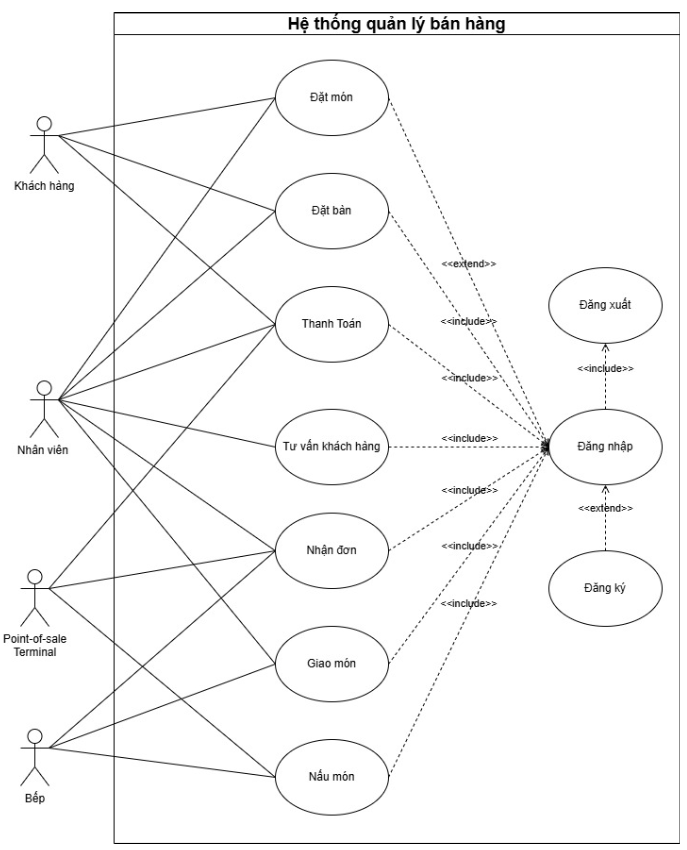
\includegraphics[width=0.8\textwidth]{task13.png}
        \caption{Use case đặt món}
    \end{figure}
    \begin{itemize}
        \item Đặc tả use case
    \end{itemize}
\begin{table}[!htbp]
\centering
\begin{tabular}{|l|p{10cm}|}
\hline
Mục & Nội dung \\
\hline
Tóm tắt & Khách hàng quét mã QR để xem menu và đặt món trực tiếp trên hệ thống. \\
\hline
Actor & Khách hàng \\
\hline
\textbf{Dòng sự kiện chính} & \\
\hline
Bước 1 & Khách hàng mở app hoặc camera trên điện thoại để quét mã QR tại bàn (Quét QR). \\
\hline
Bước 2 & Hệ thống xác thực mã QR và hiển thị giao diện menu của quán (Xem menu). \\
\hline
Bước 3 & Khách hàng lướt xem menu và chọn các món muốn ăn (Chọn món).\\
\hline
Bước 4 & Khách hàng thêm các món đã chọn vào giỏ hàng ảo trên hệ thống (Thêm món vào giỏ hàng). \\
\hline
Bước 5 & Khách hàng kiểm tra lại giỏ hàng (số lượng, món ăn) và nhấn nút xác nhận để gửi đơn hàng (Đặt món). \\
\hline
Bước 6 & Hệ thống kiểm tra tính hợp lệ của đơn hàng (ví dụ: món còn không, số lượng hợp lệ). \\
\hline
Bước 7 & Hệ thống lưu thông tin đơn hàng vào database. \\
\hline
Bước 8 & Hệ thống gửi thông báo đặt hàng thành công cho khách hàng và chuyển thông tin đơn hàng đến bộ phận bếp/pha chế.\\
\hline
Bước 9 (Tùy chọn) & Hệ thống có thể chuyển sang giao diện thanh toán hoặc chờ thanh toán sau. \\
\hline
\textbf{Dòng sự kiện phụ} & \\
\hline
3a & Mã QR không hợp lệ: Hệ thống hiển thị thông báo lỗi "Mã QR không hợp lệ" hoặc "Không tìm thấy menu".\\
\hline
5a & Món ăn hết hàng: Khi khách hàng chọn món đã hết, hệ thống hiển thị thông báo "Món [Tên món] đã hết hàng". \\
\hline
8a & Lỗi hệ thống khi đặt hàng: Nếu có lỗi xảy ra trong quá trình xử lý đơn hàng (mất kết nối, lỗi server,...), hệ thống hiển thị thông báo lỗi và yêu cầu khách hàng thử lại. \\
\hline
5b & Khách hàng muốn sửa giỏ hàng: Khách hàng có thể quay lại bước chọn món hoặc chỉnh sửa số lượng/xóa món trong giỏ hàng trước khi xác nhận. Đổi ý cái nhẹ. \\
\hline
\textbf{Tiền điều kiện} & \\
\hline
& Khách hàng phải có điện thoại thông minh có camera và kết nối internet. Đồ nghề phải đủ nha. \\
\hline
& Mã QR của quán ăn phải có sẵn và hợp lệ. \\
\hline
& Hệ thống đặt món của quán đang hoạt động bình thường. \\
\hline
\textbf{Hậu điều kiện} & \\
\hline
& Đơn hàng của khách hàng được ghi nhận thành công vào hệ thống. \\
\hline
& Khách hàng nhận được thông báo xác nhận đơn hàng trên ứng dụng/trình duyệt. \\
\hline
& Thông tin đơn hàng được chuyển đến các bộ phận liên quan (bếp, thu ngân) để xử lý.\\
\hline
\end{tabular}
\caption{Bảng mô tả quy trình khách hàng đặt món bằng mã QR}
\label{tab:dat_mon_qr}
\end{table}
    
    
\newpage
\section{TASK 2. MÔ HÌNH HÓA HỆ THỐNG}

\subsection{Task 2.1 Sơ đồ hoạt động}
Viết nội dung ở đây

\subsection{Task 2.2 Sơ đồ trình tự}
    \begin{figure}[H]
        \centering
        \includegraphics[width=1.0\textwidth]{task221.png}
        \caption{Sơ đồ trình tự tổng quan}
    \end{figure}
    \begin{figure}[H]
        \centering
        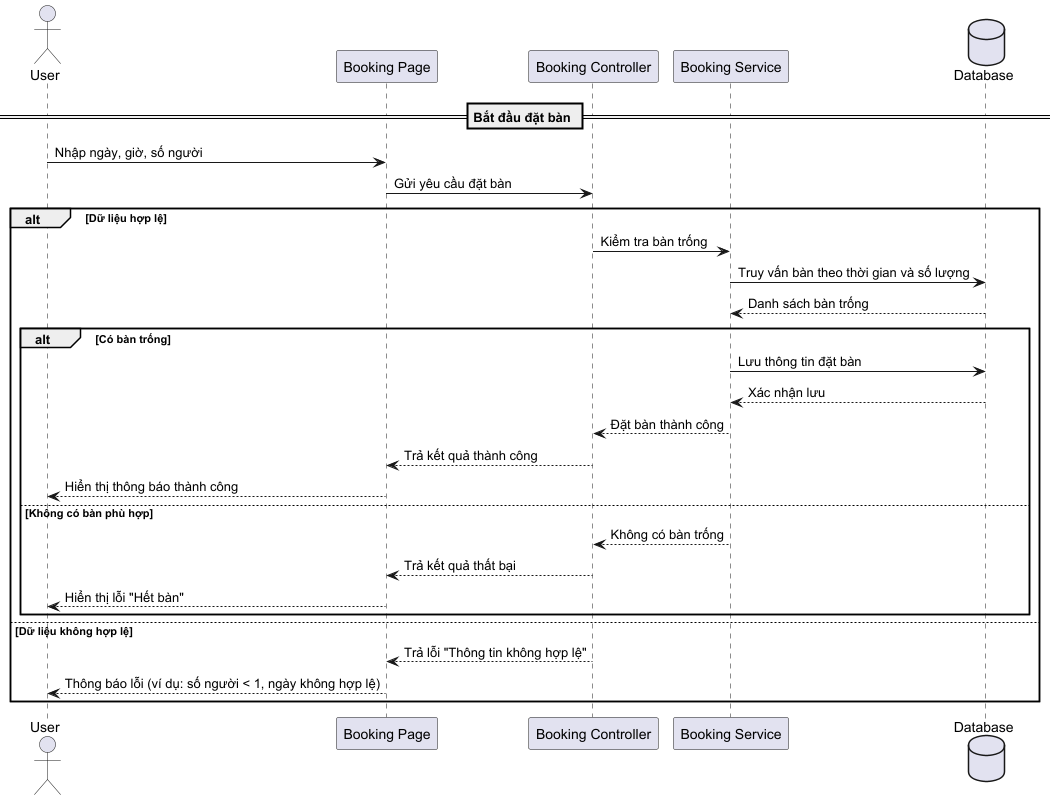
\includegraphics[width=1.0\textwidth]{task22.png}
        \caption{Sơ đồ trình tự chức năng đặt bàn}
    \end{figure}

\subsection{Task 2.3 Sơ đồ lớp}
    \begin{figure}[H]
        \centering
        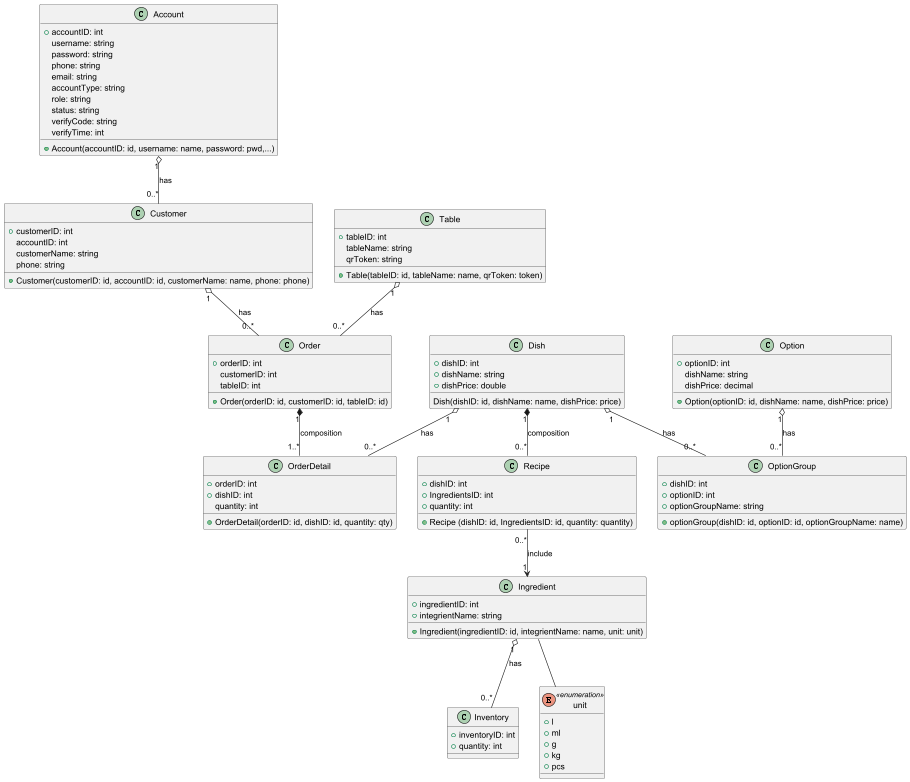
\includegraphics[width=1.0\textwidth]{task23.png}
        \caption{Sơ đồ lớp}
    \end{figure}
    \begin{itemize}
        \item[-] Bảng danh sách cách lớp:
            \begin{table}[h!]
            \centering
            \begin{tabular}{|c|l|l|l|}
            \hline
            STT & Tên Lớp & Loại & Ý nghĩa / Ghi Chú \\
            \hline
            1 & Account & Lớp con người & Đại diện cho một tài khoản người dùng \\
            \hline
            2 & Table & Lớp dữ liệu & Thông tin về bàn ứng với mã QR \\
            \hline
            3 & Customer & Lớp con người & Đại diện cho một khách hàng \\
            \hline
            4 & Order & Lớp nghiệp vụ & Đại diện cho một đơn đặt hàng \\
            \hline
            5 & OrderDetail & Lớp nghiệp vụ & Chi tiết của một đơn đặt hàng \\
            \hline
            6 & Option & Lớp dữ liệu & Một tùy chọn cho sản phẩm hoặc dịch vụ \\
            \hline
            7 & OptionGroup & Lớp dữ liệu & Nhóm các tùy chọn liên quan \\
            \hline
            8 & Dish & Lớp dữ liệu & Một món ăn trong thực đơn \\
            \hline
            9 & Recipe & Lớp dữ liệu & Công thức chế biến một món ăn \\
            \hline
            10 & Ingredients & Lớp dữ liệu & Các thành phần nguyên liệu \\
            \hline
            11 & Inventory & Lớp dữ liệu & Thông tin về kho hàng \\
            \hline
            \end{tabular}
            \caption{Bảng mô tả các lớp}
            \label{tab:cac_lop}
            \end{table}
    \end{itemize}

\newpage
\section{TASK 3. THIẾT KẾ KIẾN TRÚC}

\subsection{Task 3.1. Thiết kế kiến trúc}

\subsubsection{3.1.1. Giới thiệu}
\begin{itemize}
    \item[-]Kiến trúc phần mềm đóng vai trò là nền tảng cốt lõi, ảnh hưởng trực tiếp đến khả năng phát triển, bảo trì, và mở rộng của hệ thống "Ứng dụng Đặt hàng \& Nhà hàng". Trong dự án này, nhóm phát triển đã quyết định áp dụng kiến trúc 3 tầng (3-tier Architecture). Lựa chọn này nhằm mục đích phân tách một cách rõ ràng các khối chức năng chính của ứng dụng, từ đó tạo điều kiện thuận lợi cho việc quản lý, phát triển và kiểm thử độc lập từng thành phần. Kiến trúc 3 tầng không chỉ giúp tăng cường tính module hóa, mà còn cho phép dễ dàng nâng cấp hoặc thay thế các công nghệ ở mỗi tầng mà không gây ảnh hưởng lớn đến toàn bộ hệ thống. Đồng thời, nó cũng hỗ trợ hiệu quả cho việc cộng tác trong nhóm phát triển, khi các thành viên có thể tập trung chuyên môn vào các tầng cụ thể (ví dụ: giao diện người dùng, logic nghiệp vụ, hoặc quản lý dữ liệu).
\end{itemize}

\subsubsection{3.1.2. Phương pháp kiến trúc}
\begin{itemize}
    \item Hệ thống "Ứng dụng Đặt hàng \& Nhà hàng" được thiết kế và triển khai dựa trên mô hình kiến trúc 3 tầng (3-tier Architecture), một mô hình phổ biến và đã được chứng minh hiệu quả trong việc xây dựng các ứng dụng web hiện đại. Ba tầng chính bao gồm:
    \begin{itemize}
    \item \textbf{Tầng Trình Bày (Presentation Tier):} 
    \begin{itemize}
        \item [+]Là giao diện người dùng, nơi khách và nhân viên tương tác trực tiếp.
        \item [+] Xây dựng bằng Next.js, hiển thị thông tin trực quan, thu thập input (như đặt món, đặt bàn) và gửi yêu cầu xử lý xuống backend.
        \item [+] Gồm các trang như: đặt món qua QR, quản lý đơn hàng, menu,....
    \end{itemize}

    \item \textbf{Tầng Ứng Dụng (Application Tier / Business Logic Tier):} 
    \begin{itemize}
        \item [+] Là "bộ não" của hệ thống, phát triển bằng NestJS.
        \item [+] Xử lý toàn bộ logic nghiệp vụ: kiểm tra đơn hàng, tính tiền, khuyến mãi, đặt bàn, thống kê,...
        \item [+] Điều phối dữ liệu giữa UI và database.
    \end{itemize}

    \item [+] \textbf{Tầng Dữ Liệu (Data Tier):} 
    \begin{itemize}
        \item [+]Lưu trữ và truy xuất dữ liệu bằng MongoDB (NoSQL).
        \item [+]Đảm bảo thao tác CRUD hiệu quả, linh hoạt, phù hợp với hệ thống có dữ liệu biến đổi nhanh.
        \item [+]Đảm bảo tính toàn vẹn, bảo mật và nhất quán thông tin.
    \end{itemize}
\end{itemize}
\end{itemize}

\textbf{Luồng tương tác giữa các tầng:}
\begin{enumerate}
    \item Người dùng (khách hàng hoặc nhân viên) tương tác với các thành phần giao diện trên Tầng Trình Bày (ví dụ: nhấn nút đặt món, điền form đăng ký).
    \item Tầng Trình Bày tạo và gửi các yêu cầu (thường là các HTTP requests đến API endpoints) tới Tầng Ứng Dụng.
    \item Tầng Ứng Dụng tiếp nhận yêu cầu, xác thực (nếu cần), xử lý logic nghiệp vụ tương ứng. Trong quá trình này, Tầng Ứng Dụng có thể cần truy vấn hoặc cập nhật dữ liệu bằng cách gửi yêu cầu đến Tầng Dữ Liệu.
    \item Tầng Dữ Liệu thực thi các yêu cầu từ Tầng Ứng Dụng và trả kết quả về (ví dụ: danh sách món ăn, thông tin đơn hàng đã lưu).
    \item Tầng Ứng Dụng nhận phản hồi từ Tầng Dữ Liệu, hoàn tất việc xử lý và gửi kết quả (thường là dữ liệu dưới dạng JSON) trở lại Tầng Trình Bày.
    \item Tầng Trình Bày nhận dữ liệu, cập nhật giao diện và hiển thị thông tin cho người dùng.
\end{enumerate}

Việc lựa chọn kiến trúc 3 tầng mang lại nhiều lợi ích như: sự phân tách rõ ràng các mối quan tâm (separation of concerns), cho phép các nhóm phát triển có thể làm việc độc lập và song song trên các tầng khác nhau; tăng khả năng bảo trì và kiểm thử do các thành phần được cô lập; và cung cấp khả năng mở rộng linh hoạt cho từng tầng khi nhu cầu hệ thống tăng lên (ví dụ, có thể scale riêng tầng ứng dụng hoặc tầng dữ liệu mà không ảnh hưởng đến các tầng khác).


\subsection{Task 3.2. Sơ đồ triển khai}
    \begin{figure}[H]
        \centering
        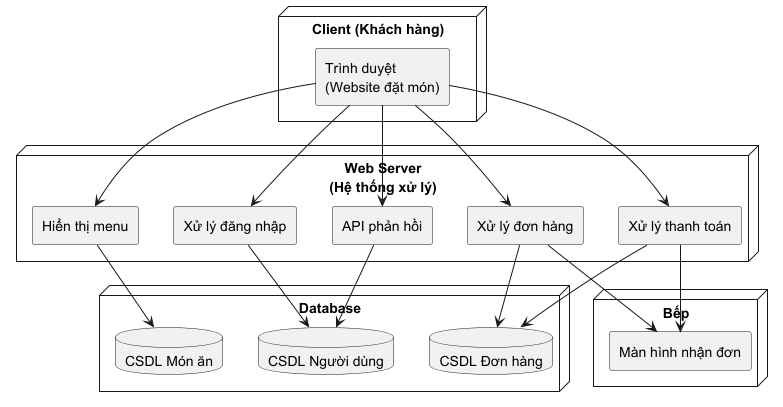
\includegraphics[width=1.0\textwidth]{task32.png}
        \caption{Sơ đồ triển khai của hệ thống}
    \end{figure}

\newpage
\section{TASK 4. TRIỂN KHAI - SPRINT 1}

\subsection{Task 4.1. Thiết lập kho lưu trữ trực tuyến}
\noindent\textbf{Link GitHub:} \href{https://github.com/Hiennguyen278610/CNPM.git}{https://github.com/CNPM.git}

\subsection{Task 4.2. Mô hình hóa hệ thống và thiết kế kiến trúc}

\subsubsection{4.2.1. Mô hình hóa hệ thống}
Viết nội dung ở đây

\subsubsection{4.2.2. Thiết kế kiến trúc}
Viết nội dung ở đây

\newpage
\section{TASK 5. TRIỂN KHAI - SPRINT 2}

\subsection{5.1. Giao diện phần mềm}

\subsubsection{5.1.1. Giao diện được thiết kế}
\begin{figure}[H]
        \centering
        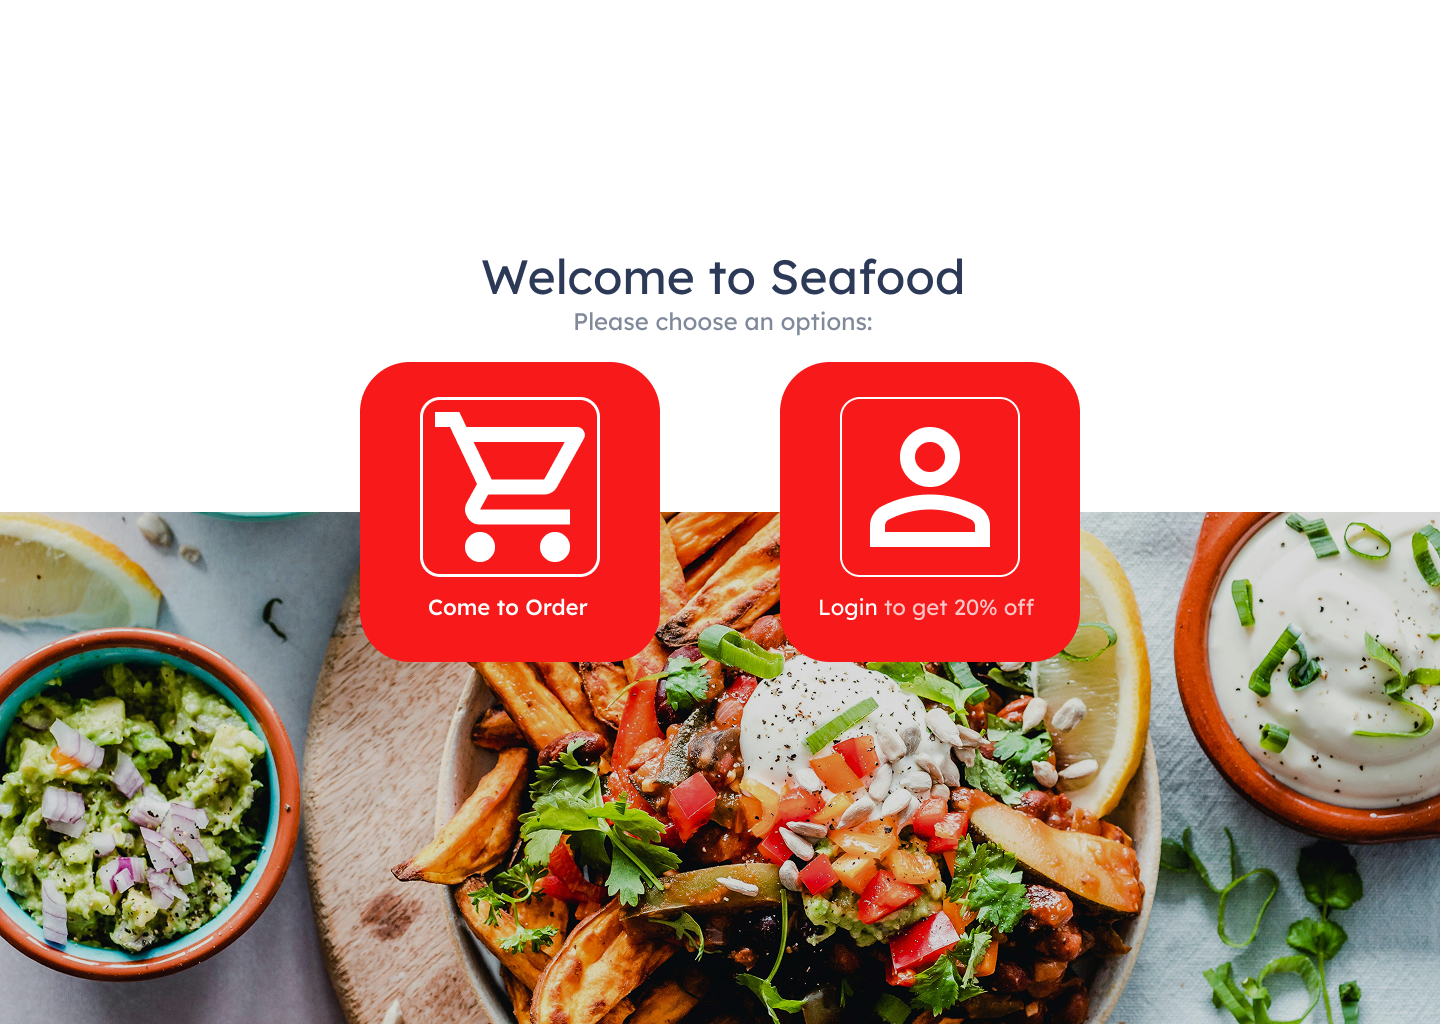
\includegraphics[width=0.8\textwidth]{figmaHome.png}
        \caption{Giao diện trang chủ - Hiển thị thông tin chào mừng và danh mục món ăn phổ biến}
    \end{figure}
    
    \begin{figure}[H]
        \centering
        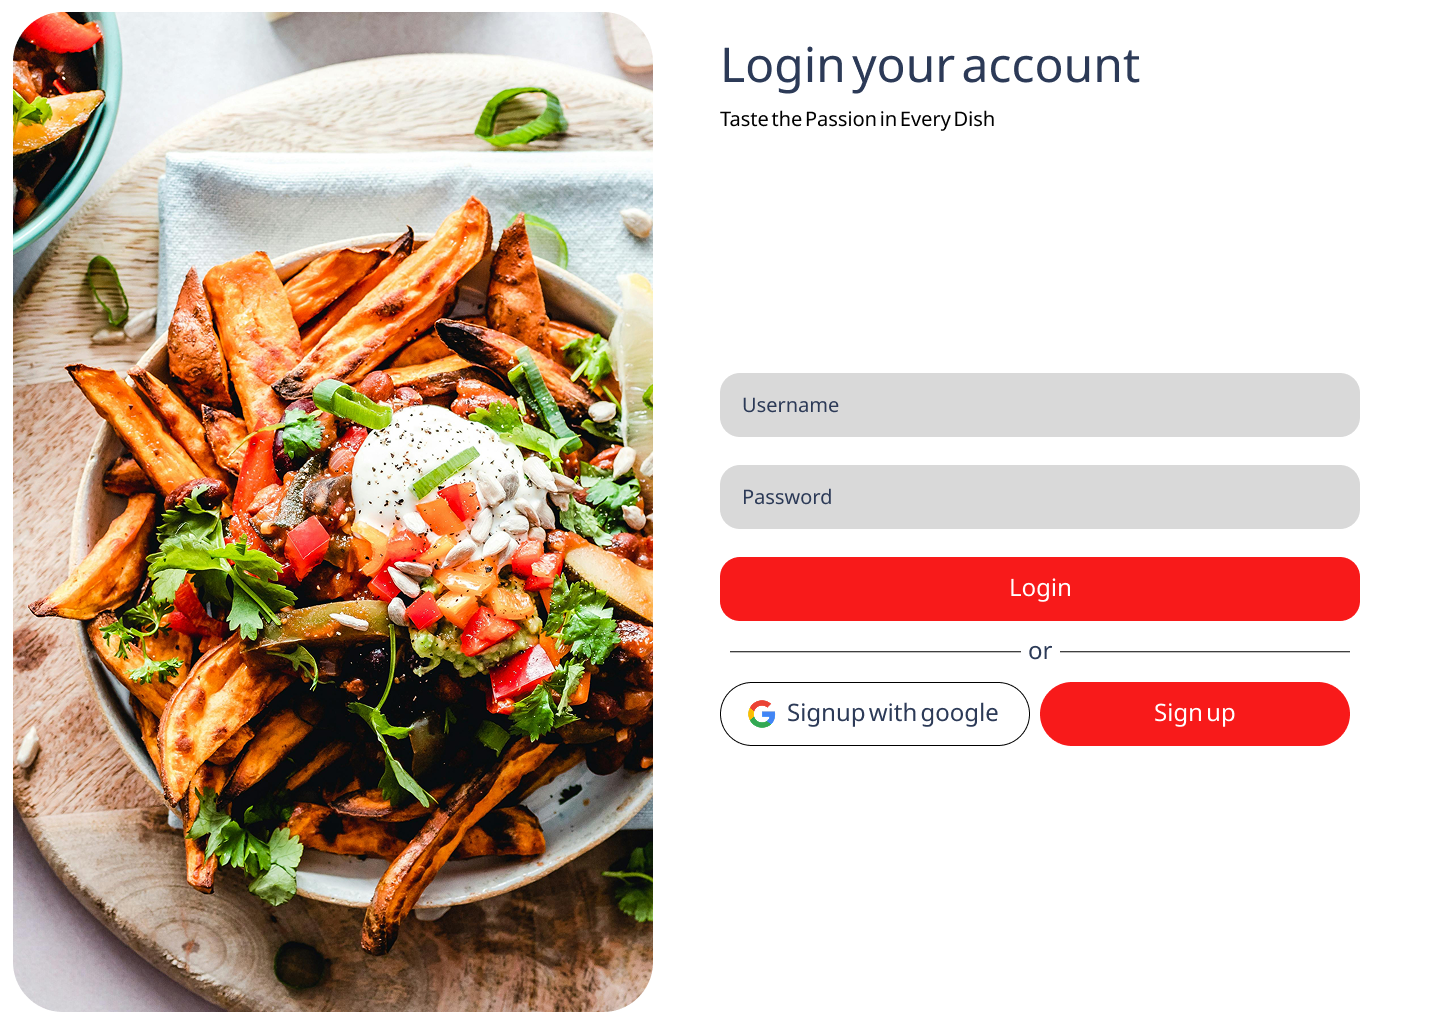
\includegraphics[width=0.8\textwidth]{figmaLogin.png}
        \caption{Giao diện đăng nhập - Cho phép người dùng đăng nhập với email và mật khẩu}
    \end{figure}
    
    \begin{figure}[H]
        \centering
        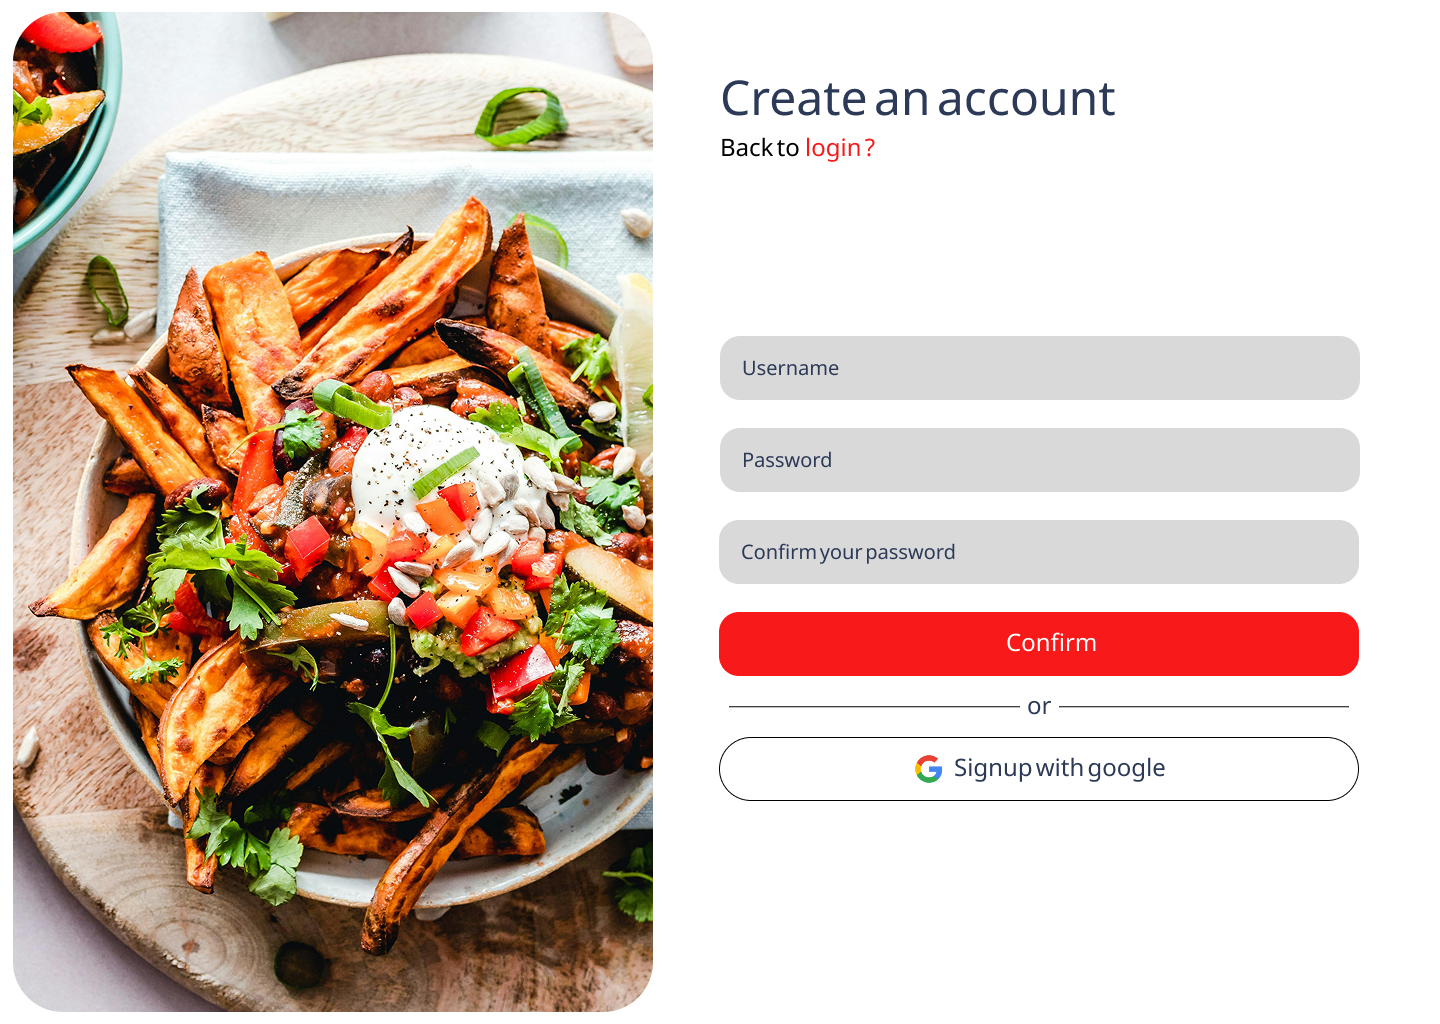
\includegraphics[width=0.8\textwidth]{figmaRegister.png}
        \caption{Giao diện đăng ký - Cho phép người dùng đăng ký tài khoản mới với thông tin cá nhân}
    \end{figure}
    
    \begin{figure}[H]
        \centering
        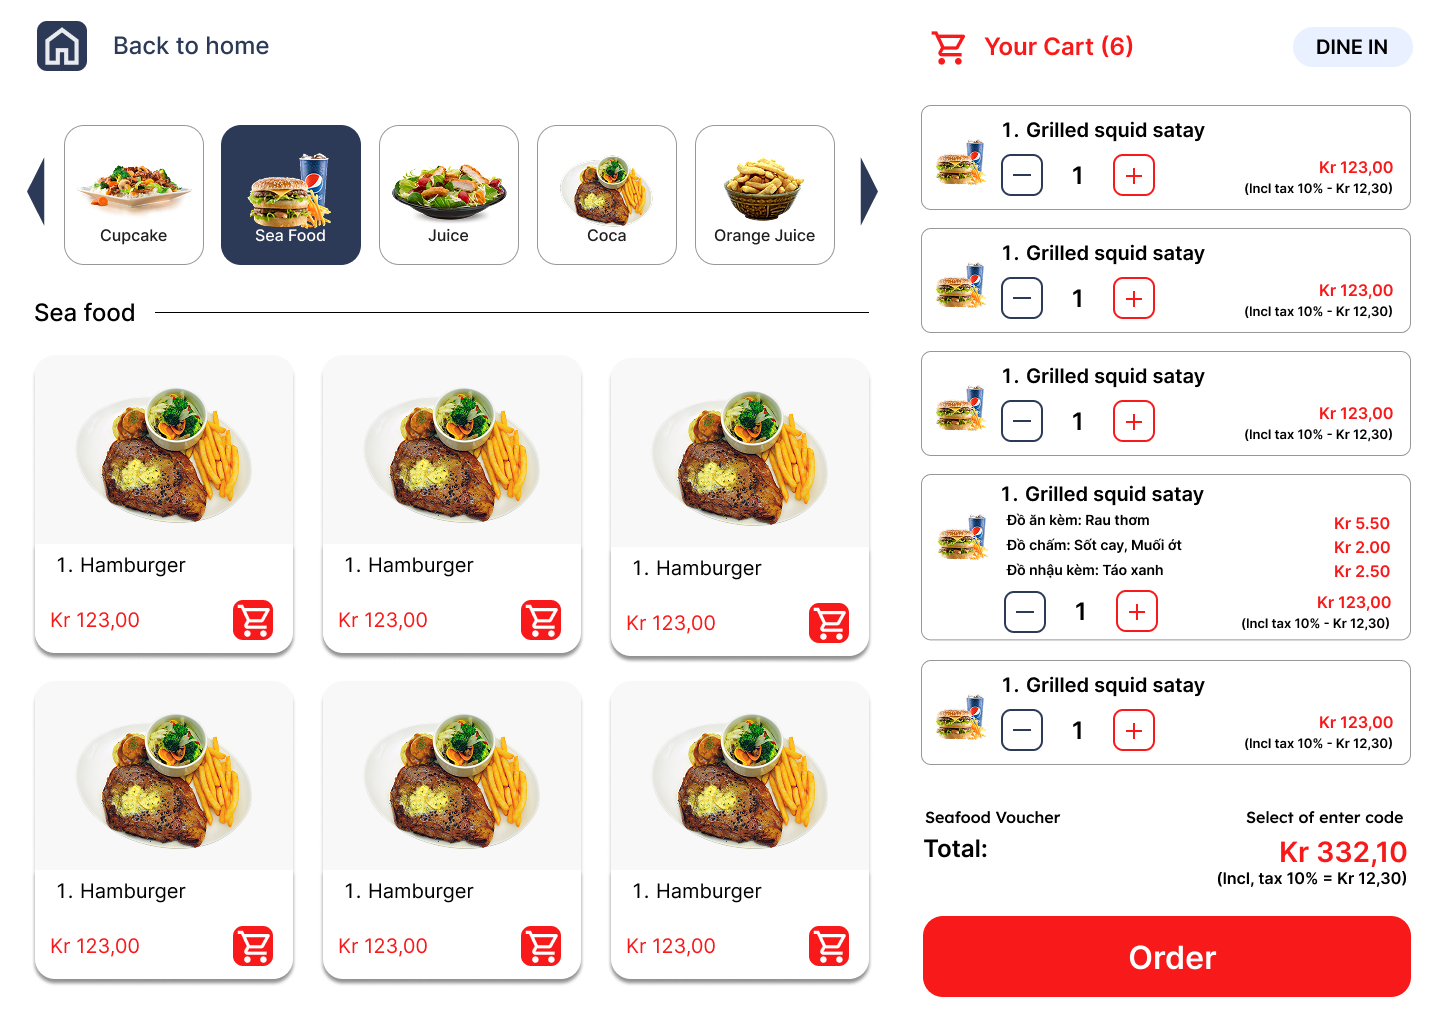
\includegraphics[width=0.8\textwidth]{figmaMenu.png}
        \caption{Giao diện thực đơn - Hiển thị danh sách các món ăn theo từng danh mục}
    \end{figure}
    
    \begin{figure}[H]
        \centering
        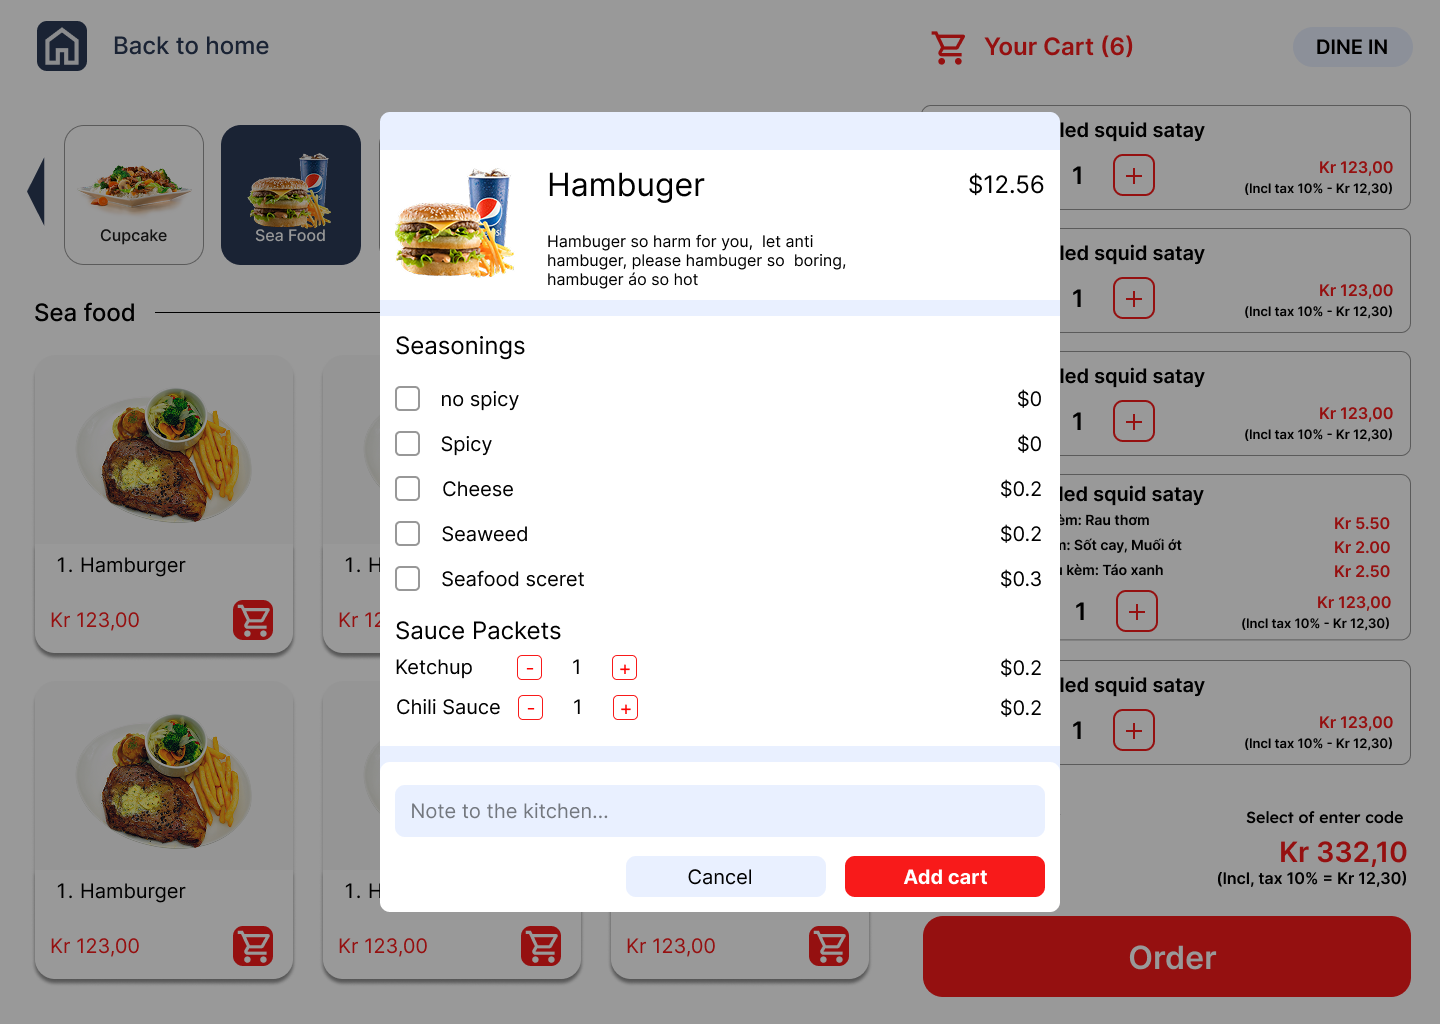
\includegraphics[width=0.8\textwidth]{figmaOrderDetail.png}
        \caption{Giao diện chi tiết đơn hàng - Hiển thị thông tin chi tiết về đơn hàng đã đặt}
    \end{figure}
    
    \begin{figure}[H]
        \centering
        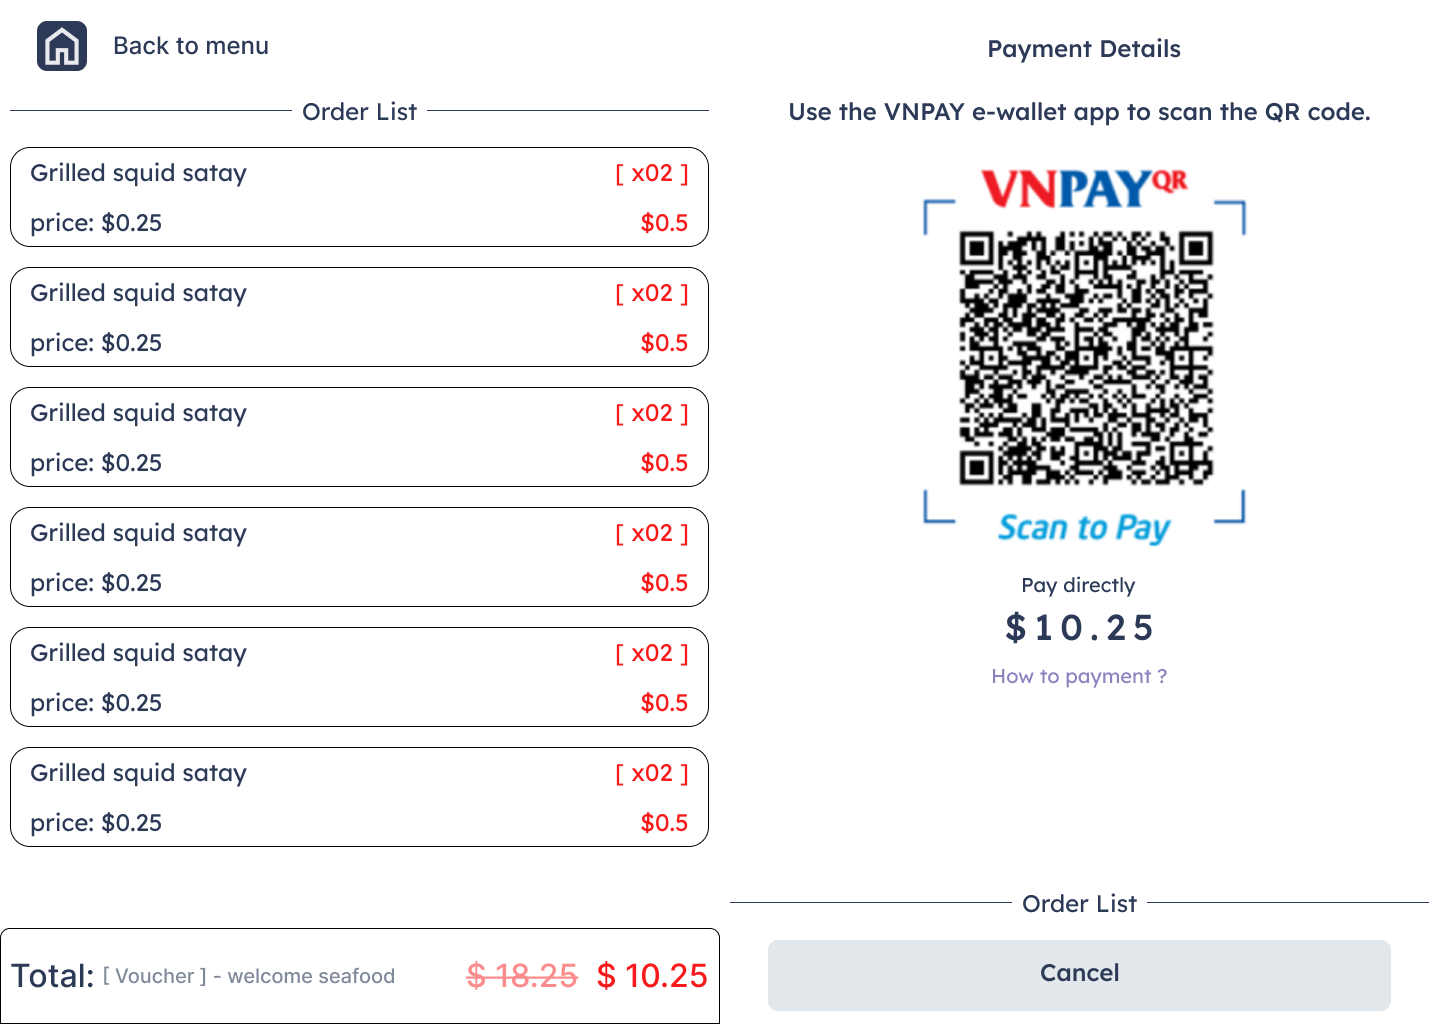
\includegraphics[width=0.8\textwidth]{figmaPayment.png}
        \caption{Giao diện thanh toán - Cho phép người dùng lựa chọn phương thức thanh toán và hoàn tất đơn hàng}
    \end{figure}

\subsubsection{5.1.2. Giao diện được triển khai}
\subsection{Giao diện được triển khai}
    \begin{figure}[H]
        \centering
        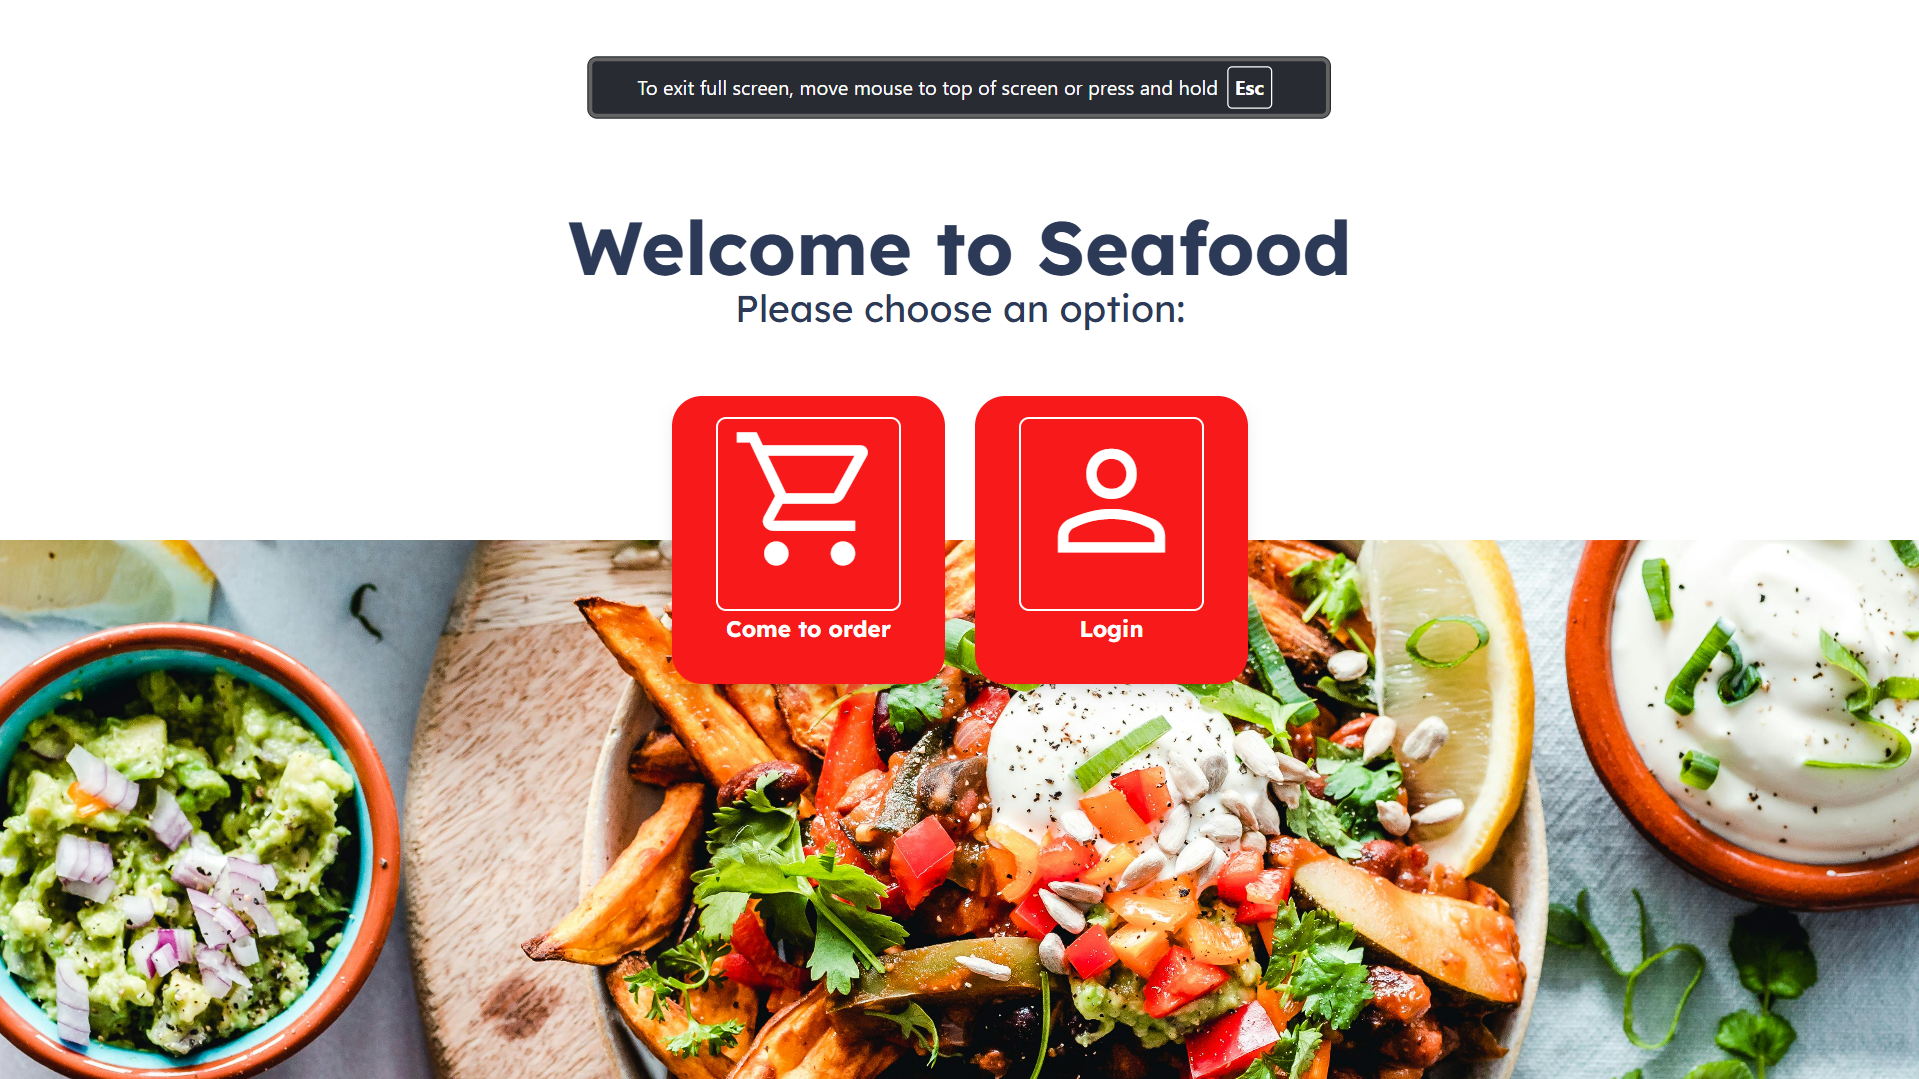
\includegraphics[width=0.8\textwidth]{home.png}
        \caption{Giao diện trang chủ - Hiển thị thông tin chào mừng và danh mục món ăn phổ biến}
    \end{figure}
    
    \begin{figure}[H]
        \centering
        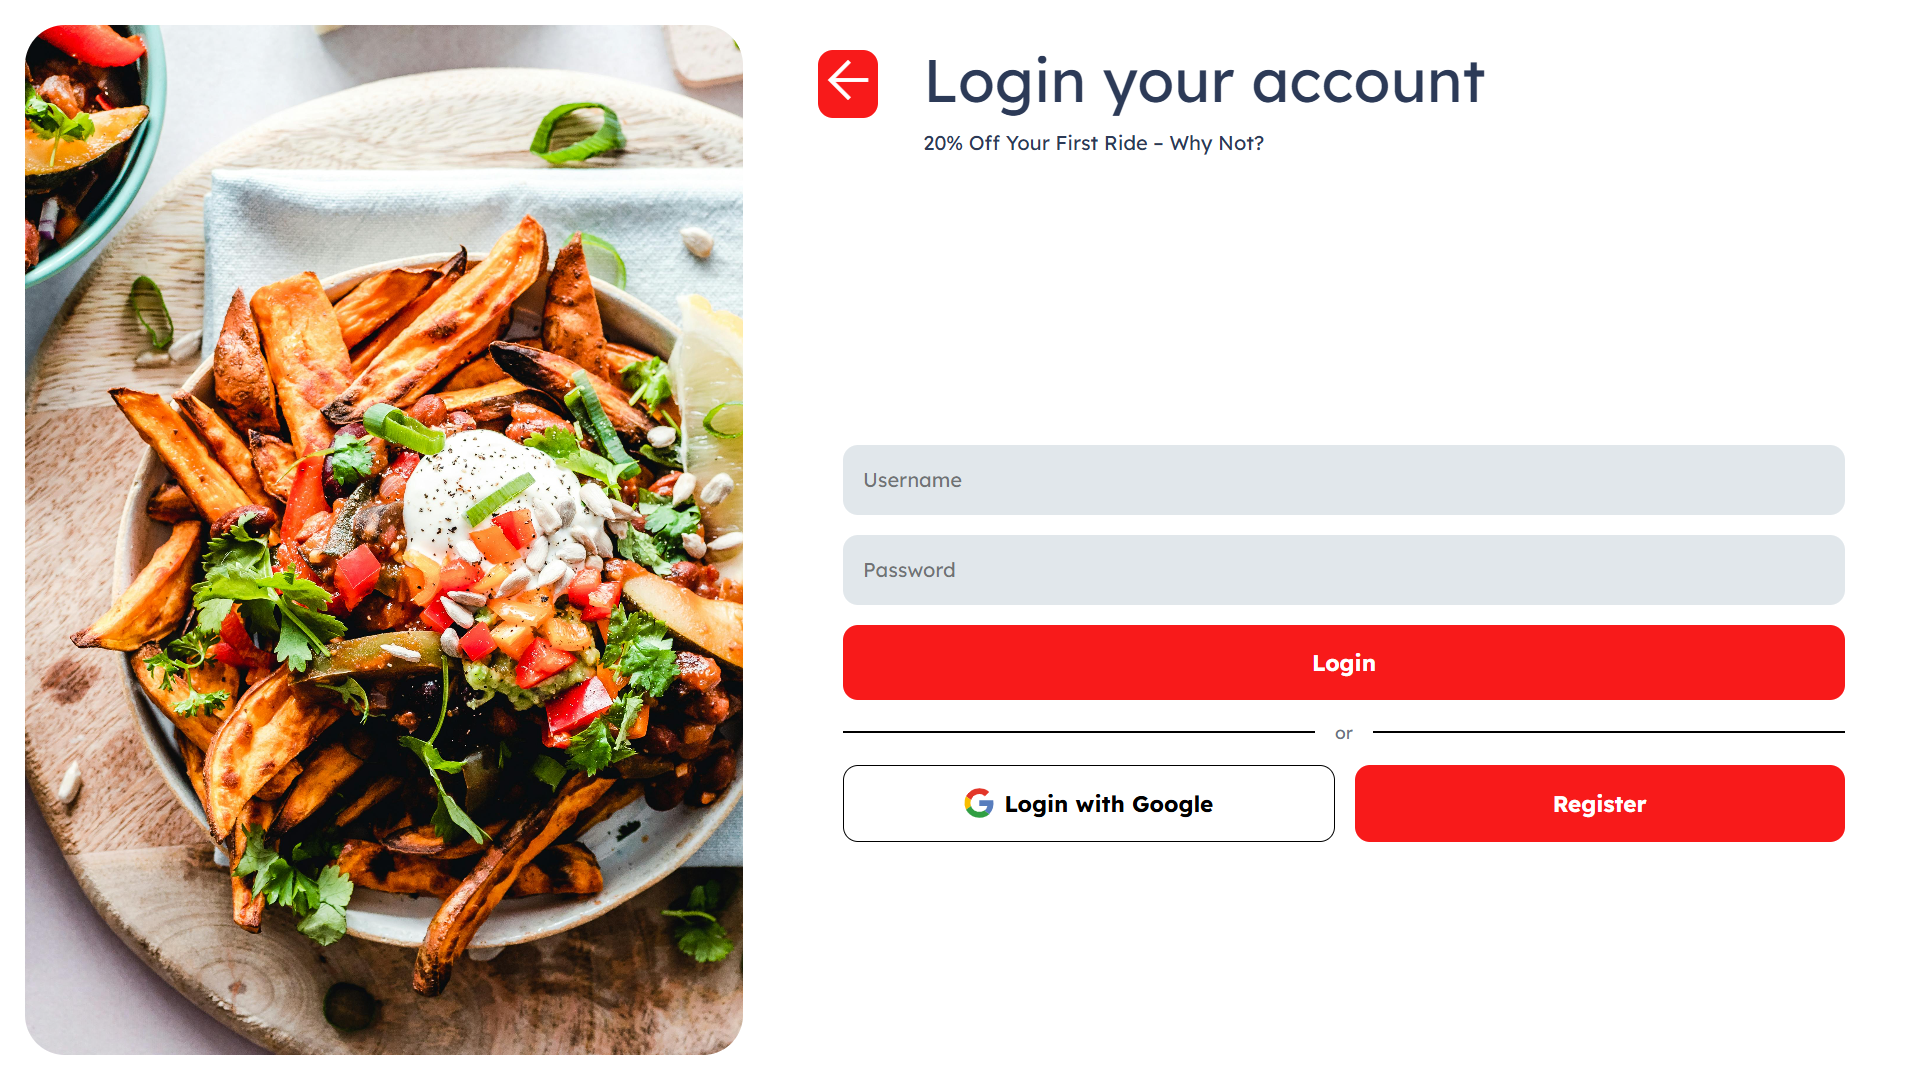
\includegraphics[width=0.8\textwidth]{login.png}
        \caption{Giao diện đăng nhập - Cho phép người dùng đăng nhập với email và mật khẩu}
    \end{figure}
    
    \begin{figure}[H]
        \centering
        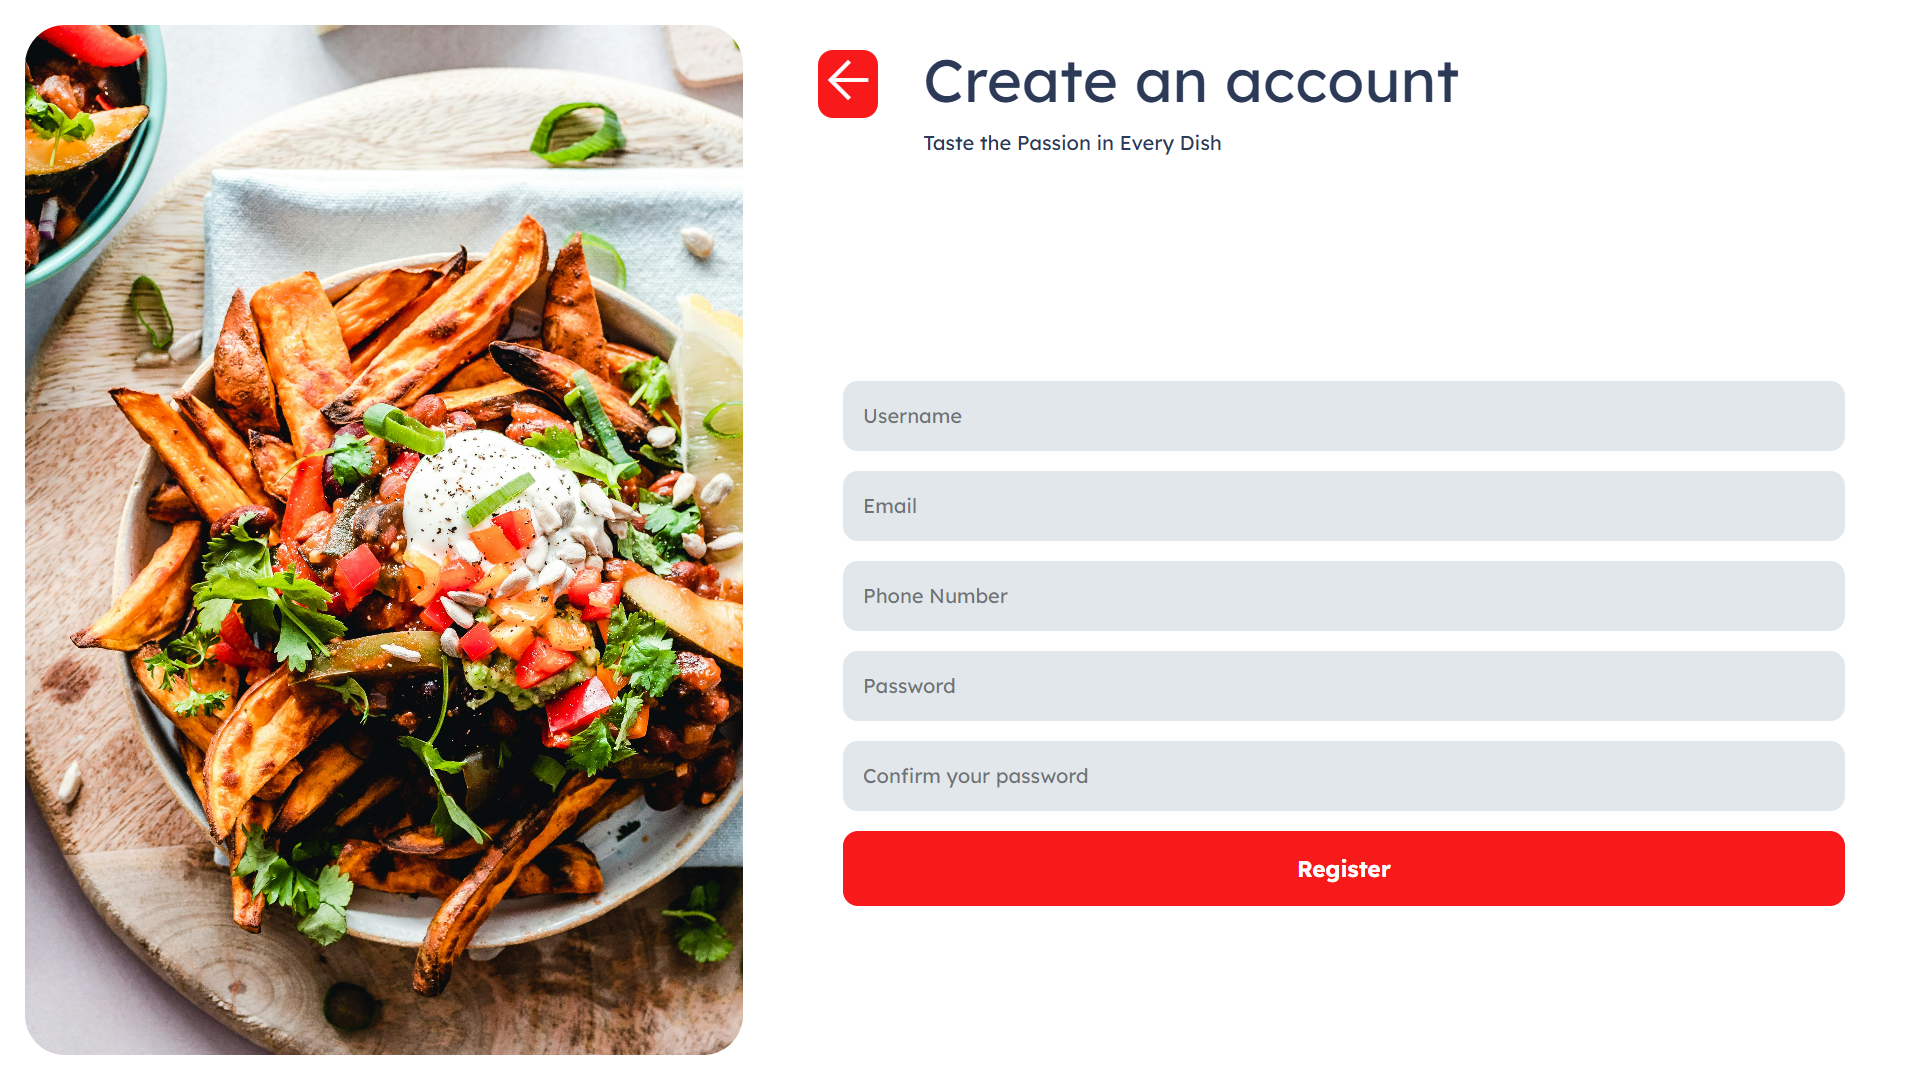
\includegraphics[width=0.8\textwidth]{register.png}
        \caption{Giao diện đăng ký - Cho phép người dùng đăng ký tài khoản mới với thông tin cá nhân}
    \end{figure}
    
    \begin{figure}[H]
        \centering
        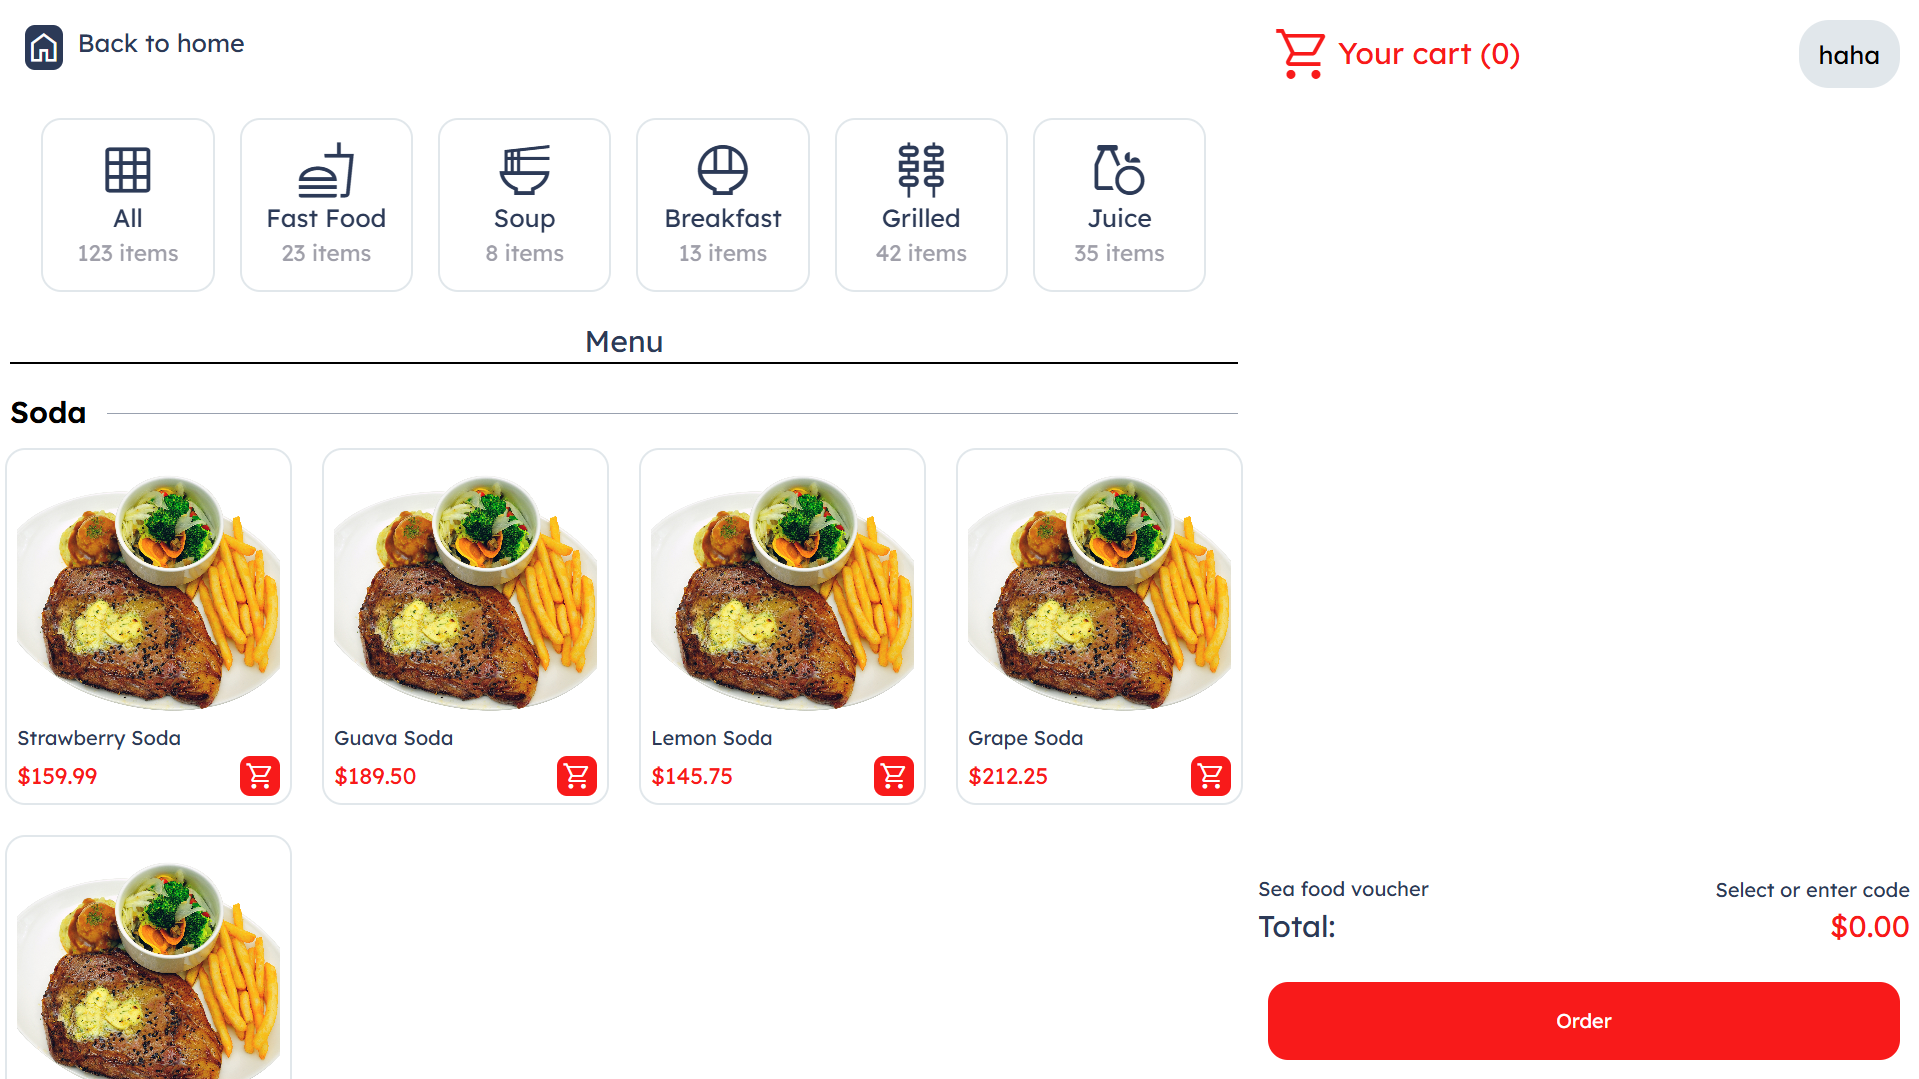
\includegraphics[width=0.8\textwidth]{menu.png}
        \caption{Giao diện thực đơn - Hiển thị danh sách các món ăn theo từng danh mục}
    \end{figure}
    
    \begin{figure}[H]
        \centering
        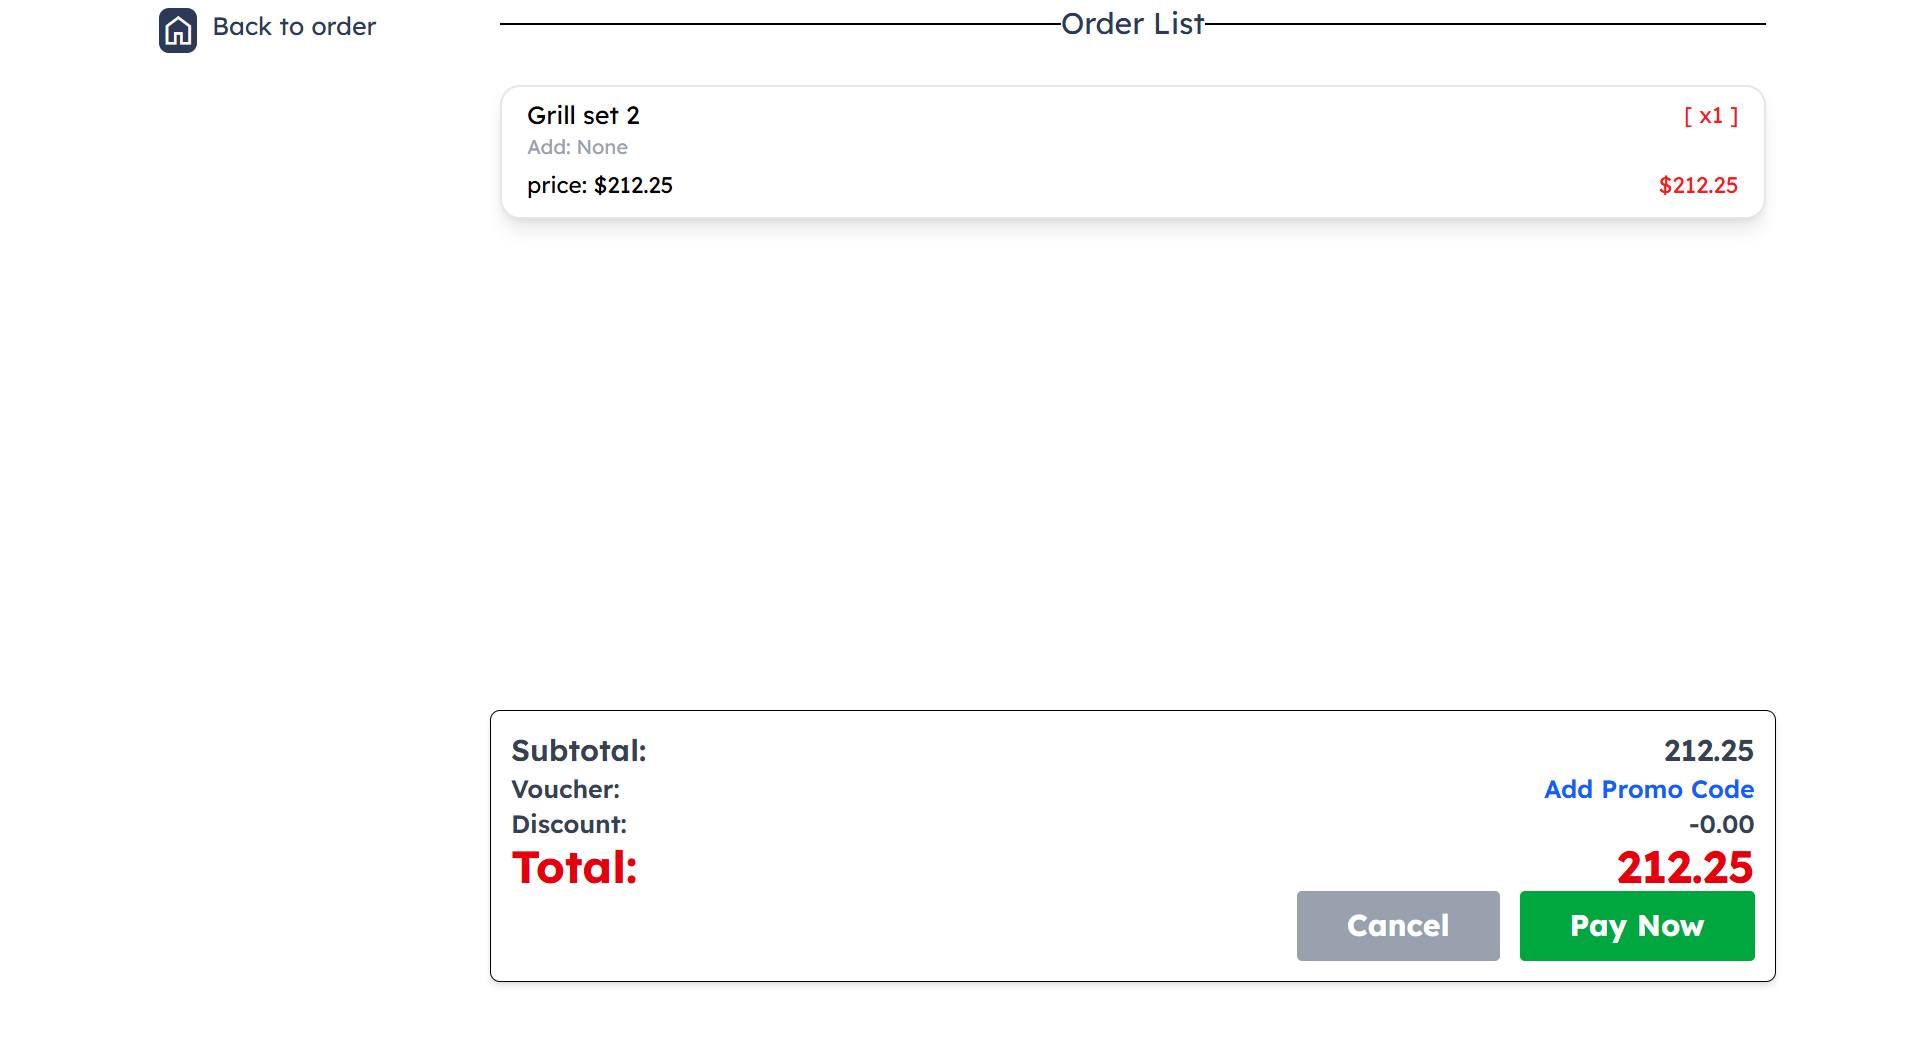
\includegraphics[width=0.8\textwidth]{payment.png}
        \caption{Giao diện thanh toán - Cho phép người dùng lựa chọn phương thức thanh toán và hoàn tất đơn hàng}
    \end{figure}

\subsection{5.2. Kiểm thử}
Viết nội dung ở đây

\newpage
\section{KẾT LUẬN}
\begin{itemize}
    \item [-] Dự án xây dựng "Ứng dụng Đặt hàng & Nhà hàng" đã hoàn thành và đạt được những mục tiêu quan trọng đặt ra ban đầu, bao gồm các yêu cầu về chức năng, hiệu năng và bảo mật. Hệ thống cung cấp một giải pháp toàn diện cho phép khách hàng dễ dàng đặt món và thanh toán qua mã QR, đồng thời hỗ trợ nhà hàng tối ưu hóa quy trình vận hành, quản lý đơn hàng, và nâng cao trải nghiệm dịch vụ. Mục tiêu thay thế POS truyền thống và đáp ứng nhu cầu mở rộng trong tương lai của nhà hàng đã được chú trọng.
    \item [-] Trong quá trình phát triển, dự án không chỉ tập trung vào việc triển khai các tính năng cốt lõi như đặt món trực tuyến, quản lý bàn, xử lý thanh toán đa dạng, và quản lý thực đơn, mà còn chú trọng đến trải nghiệm người dùng thân thiện trên các giao diện web và di động. Khả năng mở rộng của hệ thống để đáp ứng sự phát triển của nhà hàng và tính dễ bảo trì cũng là những yếu tố được ưu tiên. Những cải tiến về hiệu năng xử lý giao dịch đồng thời và các biện pháp bảo mật dữ liệu người dùng, dữ liệu giao dịch đã giúp hệ thống đáp ứng tốt nhu cầu vận hành thực tế, đồng thời sẵn sàng cho việc tích hợp thêm các tính năng mới khi hoạt động kinh doanh của nhà hàng phát triển.
    \item [-] Mặc dù dự án đã đạt được những kết quả tích cực và đáp ứng các yêu cầu đề ra, vẫn còn nhiều tiềm năng để nâng cấp và tối ưu hóa hơn nữa nhằm mang đến giá trị lớn hơn cho cả phía nhà hàng và thực khách. Các hướng phát triển có thể bao gồm việc hoàn thiện hơn nữa các module quản lý kho, phân tích dữ liệu kinh doanh thông minh để đưa ra các gợi ý chiến lược, hoặc mở rộng các chương trình khách hàng thân thiết. Đây sẽ là nền tảng vững chắc để nhóm phát triển tiếp tục nghiên cứu, cải thiện hệ thống, bổ sung các tính năng nâng cao và hoàn thiện hơn nữa sản phẩm trong các giai đoạn phát triển tiếp theo, góp phần vào sự thành công và hiện đại hóa của các mô hình kinh doanh ẩm thực.
\end{itemize}


\newpage

\begin{thebibliography}{80}

\bibitem{YT}
``\textbf{Restaurant Management System Guide}'',
\textit{Youtube Video Reference}, 
\textbf{link: https://www.youtube.com/watch?v=5Ul\_rUuoUZE},
lần truy cập cuối: 01/05/2024.

\bibitem{NEXT}
Next.js Documentation,
``\textbf{link: https://nextjs.org/docs}'',
\textit{The React Framework for the Web},
lần truy cập cuối: 03/05/2024.

\bibitem{NEST}
NestJS Documentation,
``\textbf{link: https://docs.nestjs.com/}'',
\textit{A progressive Node.js framework},
lần truy cập cuối: 03/05/2024.

\bibitem{MONGO}
MongoDB Documentation,
``\textbf{link: https://www.mongodb.com/docs/}'',
\textit{MongoDB Documentation},
lần truy cập cuối: 03/05/2024.

\bibitem{DOCKER}
Docker Documentation,
``\textbf{link: https://docs.docker.com/}'',
\textit{Docker Documentation},
lần truy cập cuối: 03/05/2024.

\bibitem{REACTJS}
React Documentation,
``\textbf{link: https://react.dev/reference/react}'',
\textit{A JavaScript library for building user interfaces},
lần truy cập cuối: 05/05/2024.

\bibitem{TAILWIND}
Tailwind CSS Documentation,
``\textbf{link: https://tailwindcss.com/docs}'',
\textit{A utility-first CSS framework},
lần truy cập cuối: 05/05/2024.

\bibitem{NPM}
npm Documentation,
``\textbf{link: https://docs.npmjs.com/}'',
\textit{The world's largest software registry},
lần truy cập cuối: 05/05/2024.

\bibitem{SWIPER}
Swiper Documentation,
``\textbf{link: https://swiperjs.com/get-started}'',
\textit{The Most Modern Mobile Touch Slider},
lần truy cập cuối: 05/05/2024.

\end{thebibliography}
\end{document}
